\chapter{Einleitung} \label{Einleitung}
Der Anteil von in Ballungsräumen lebenden Personen wird immer größer. Während 1990 noch 43\% der Welt in Ballungsräumen lebte, ist diese Prozentzahl bis 2015 auf 53.9\% angestiegen (\cite{UnitedNations.2018}). Da ein großer Anteil der Personen, die in diesen Räumen lebt, öffentliche Verkehrsmittel nutzt, sind in diesen höhere Passagierzahlen zu  erwarten. Durch diesen Wandel wird es immer wichtiger, den öffentlichen Nahverkehr effizient zu gestalten und eine schnelle Evakuierung in Gefahrenfällen sicherzustellen. Vor allem zu den Spitzenzeiten ist die Effizienz ein wichtiger Faktor für ein gutes Fahrerlebnis.

Eine Simulation, die die notwendigen Haltezeiten von Zügen mithilfe von realistischen Fahrgastwechselmodellen ermittelt, kann zu einer Verbesserung des öffentlichen Personennahverkehrs führen. Die Ergebnisse einer Simulation könnten die Grundlage für die Fahrplan-Planung bilden.

Um die Grundlage für eine solche Simulation zu erhalten, beobachte und untersuche ich in dieser Arbeit das Verhalten von Personen beim Fahrgastwechsel an U-Bahn-Stationen. Aus den gesammelten Daten leite ich ein Modell ab, dass den Fahrgastwechsel an Zügen realistischer abbilden soll.

Im folgenden Abschnitt wird der Stand der Technik und die daraus folgende Motivation für diese Arbeit beschrieben.
\section{Stand der Technik} \label{Stand der Technik}
Um passende Literatur zu finden suchte ich in der Bibliothek der Hochschule München, Google Scholar, sowie Scopus. Hierbei verwendete ich die Suchbegriffe "`Fahrgastwechsel"', "`Einsteigen"', "`Aussteigen"', "`passenger exchange"', "boarding"' und "`alight"' in Kombination mit "`Öffentliche Verkehrsmittel"', "`Bahnhof"', "`U-Bahn"', "`public transport"', "`station"', "`metro"', "`subway"' und "`railway"'.

Bei dieser Suche fand ich einige Studien zur Modellierung von Personen in öffentlichen Verkehrsnetzen.
Eine Untersuchung an zwei Bahnhöfen in Deutschland beschäftigt sich mit der Einführung von Wartezonen, um Personenstromsimulationen von Bahnsteigen zu verbessern (\cite{Davidich.2013}). Hierbei wurden zunächst empirische Daten dazu gesammelt, wie Personen, die aus einem Zug aussteigen, sich durch eine wartende Menge bewegen. Ein Vergleich dieser Daten mit den Ergebnissen von Simulationen mit Wartezonen, führte zu der Erkenntnis, dass die Einflüsse von wartenden Personen mit diesem Modell realistisch dargestellt werden können. \\
Ein weiterer Artikel beschäftigt sich mit Simulationen von Stationen mit vorhandener Software und dem Vergleich der Simulationen. Hierbei wird sowohl kommerzielle als auch Open-Source-Software verwendet (\cite{DubrocaVoisin.2019}). Die Modelle, welche von den Programmen verwendet werden, wurden von den Autoren jedoch nicht getestet. Somit kommen diese zu dem Schluss, dass diese Modelle näher untersucht werden müssen. Zudem erklären Sie das eine genauere Identifizierung von Verhaltensweisen im Kontext des öffentlichen Nahverkehrs stattfinden muss.\\
Abgesehen von den Simulationen von \cite{DubrocaVoisin.2019} wurde auch der Personenstrom in einer Bahnhofshalle während des Frühlingsfests an der Hangzhou Bahnstation untersucht (\cite{Wang.2013}). Dieser Artikel beschäftigt sich mit einer Modifikation des "`social force"' Modells, bezieht sich dabei jedoch nicht im speziellen auf die Umgebung des Bahnhofes. Ein weiterer Teil dieser Untersuchung beschäftigte sich zudem mit Strategien für Travel-Management. Bei ihrer Untersuchung kamen \cite{Wang.2013} zu vier Ergebnissen. Zum einen, dass die Anzahl der Passagiere ein signifikanter Faktor für die Evaluierungszeit ist. Zum anderen, dass auch das Schema der Fahrkartenüberprüfung einen Einfluss auf die vergehende Zeit hat. Zudem kamen die Wissenschaftler zu dem Schluss, dass sich die Geschwindigkeit verringert, wenn Personen große Gepäckstücke mit sich tragen. Die Ergebnisse werden in dieser Studie als guter Ansatz für weitere Untersuchungen gesehen. \\
Auch eine Fußgängersimulation für eine U-Bahn-Station wurde schon untersucht (\cite{Chen.2017}). Hierbei wird nicht nur der Bahnsteig simuliert, sondern ein gesamter Bahnhof, mit Aufzügen, Türen, Service- und Infostellen. Das Ein- und Aussteigen am Zug wird in diesem Modell wie das Gehen durch eine Tür behandelt. Die Autoren dieser Arbeit merken an, dass noch nicht jedes Verhalten der Passagiere ausreichend bewertet wurde. Deshalb wäre es noch nötig weitere Verhaltensweisen zu integrieren. Zudem sollten noch sensitive Analysen und empirische Untersuchungen durchgeführt werden, um eine robuste und präzise Simulation sicher stellen zu können. \\
Eine Simulation von Passagieren in einem gesamten Bahnnetz wurde ebenfalls schon beschrieben (\cite{Albert.2018}). \cite{Albert.2018} beziehen sich hier vor allem auf durch Passagiere verursachte Verspätungen. Als Ergebnis dieser Studie wurde angegeben, dass ein großer Faktor für Verspätungen das Verhalten der Passagiere ist. In Ihrem Fazit geben die Autoren deshalb an, dass weiterführenden Untersuchungen zum Verhalten der Fahrgäste angestellt werden sollten. \\
Alle genannten Studien beziehen sich somit auf Fußgängersimulationen im öffentlichen Nahverkehr stellen jedoch kein befriedigendes Modell für den Fahrgastwechsel vor.

Ich fand jedoch auch Artikel, welche sich genauer mit dem Fahrgastwechsel beschäftigen. Eine empirische Untersuchung aus England beschäftigt mit der Voraussage wie lange ein Zug an einem Bahnsteig steht (\cite{Harris.2006}). Dabei geht \cite{Harris.2006} auf Parameter ein, die \zB beschreiben, wie viele Personen ein- und aussteigen oder wie viele Türen es gibt. Bei ihm wird der Entscheidungsprozess einzelner Personen somit außer Acht gelassen. Bei den Untersuchungen der Ein- und Ausstiegsraten kam \cite{Harris.2006} zu dem Ergebnis, dass diese nicht für alle Passagiere einer Gruppe konstant sind. \\
Ein Modell, welches einzelne Agenten und ihre Entscheidungsfindung beschreibt, wurde im "`Journal of Advanced Transportation"' beschrieben (\cite{Tang.2017}). Allerdings wird hier nicht ein bidirektionaler Fahrgastwechsel betrachtet. Das Modell gilt für Züge, an denen Personen nur einsteigen und bezieht sich nur auf eine einzelne Station, die HSR-Station, in Beijing. Durch ihre Studie stellen \cite{Tang.2017} fest das die Bewegungen der Passagiere auf der Plattform maßgeblich von ihrem Zielwagon beeinflusst werden. Zudem fanden die Wissenschaftler heraus das eine ungeschickte Wahl der Tür seitens der Passagiere zu einer Verlängerung der Einstiegszeiten führt.\\
Eine Studie aus Beijing beschäftigt sich mit der Modellierung und Simulation von Passagieren auf einem mikroskopischen Level (\cite{Zhang.2008}). Das Modell von \cite{Zhang.2008} erfasst individuelle Charakteristiken und kollektives Gruppenverhalten während des Fahrgastwechsels. Sie zeigen einen Zusammenhang zwischen der durchschnittlichen Ausstiegszeit und dem anfänglichen Verhältnis der Anzahlen der Ein- und Aussteiger.

Das Verhalten von Personen in Bahnhöfen wurde also schon untersucht und modelliert. Oft wurde hierbei jedoch der Fahrgastwechsel an sich nicht genauer untersucht. Beiträge, die dies taten, und öffentlich zugänglich waren, wurden jedoch nicht in Deutschland durchgeführt. Wie \cite{Zhang.2008} in seinem Beitrag durch die Sichtung verschiedener Artikel feststellte, erzeugen Studien zum Ein- und Ausstiegsverhalten an Zügen in verschiedenen Ländern unterschiedliche Ergebnisse.
Deshalb ist es wichtig, den Fahrgastwechsel exemplarisch an Münchener U-Bahn-Stationen zu untersuchen um zu einem guten Modell für dieses Verkehrsmittel in München/Deutschland zu gelangen.
Schon in früheren Projekten hat der Auftraggeber dieser Bachelorarbeit, accu:rate, Personenströme an Zügen mit Wartezonen simuliert (nähere Beschreibung in \ref{Accurate Modell}). Ihre Modellierung des Fahrgastwechsels ist zwar plausibel, beruht jedoch nicht auf systematischen Beobachtungen. Ob und wie diese Modellierung angepasst werden muss, werde ich in dieser Arbeit untersuchen. Hierzu hole ich die empirische Beobachtung nach. Die gesammelten Daten werte ich aus und mit dieser Auswertung bilde ich ein Modell. Hierbei will ich folgende Forschungsfragen beantworten:
\begin{itemize}
 \item "`Welche Verhaltensweisen und Merkmale von Fahrgästen beeinflussen die benötigte Zeit für den Fahrgastwechsel?"'
 \item "`Welche Entscheidungen trifft der Fahrgast während des Fahrgastwechselprozesses?"'
 \item "`Kann die Fahrgastwechselzeit aus der Anzahl der Aus-, Einsteiger und Platzmacher \footnote{Definition Platzmacher in \ref{Begriffe und Definitionen}} abgeschätzt werden?"'
\end{itemize}
\section{Struktur der Arbeit} \label{Struktur der Arbeit}
Im \ref{Beobachtung}. Kapitel gehe ich auf die Beobachtungen der U-Bahnen ein. Dabei beschriebe ich wann, wo und wie die Aufnahmen der U-Bahn mit Kamera stattfanden. Ich beschreibe den Standardfall des Fahrgastwechsel. Dieser Standardfall wird mit einem beobachteten Sonderfall, das Wechselverhalten vor einem Fußballspiel in München, verglichen.\\
In Kapitel \ref{Forschungsfragen} verfeinere ich die in \ref{Stand der Technik} genannten Forschungsfragen. Diese Verfeinerung führe ich auf Grundlage einer ersten Betrachtung der Aufnahme durch. Die Fragen werde ich im Späteren durch die statistischen Auswertungen der Daten beantworten.\\
Kapitel \ref{Datenerhebung} beschreibt dann, wie ich die für die Forschungsfragen relevanten Daten aus den Videos extrahiert habe.\\
Die Auswertung des gesammelten Materials beschreibe ich im \ref{Datenauswertung}. Kapitel. Hierbei werte ich die Daten statistisch aus und treffe eine Entscheidung darüber, welche Merkmale und Verhaltensweisen in das Modell mit eingehen.\\
Das Modell wird stelle ich dann in Kapitel \ref{Modell} dar. Zunächst stelle ich ein Modell für den Fahrgastwechsel auf. Daraufhin beschreibe ich ein Algorithmus, mit dem dieses umgesetzt werden kann. Zum Schluss erkläre ich die Parameter, welche für das Modell relevant sind. \\
Im letzten Kapitel, Kapitel \ref{Fazit und Ausblick}, ziehe ich dann ein Fazit über die Arbeit und das Modell und gebe einen Ausblick, wie dieses Modell in Personenstromsimulationen eingesetzt werden könnte.
Die Struktur dieser Arbeit beruht auf meinem Vorgehen zur Modellfindung. Dieses Vorgehen kann in \figurename \ref{fig:Vorgehen} betrachtet werden.
\begin{figure}[H]
	\centering
		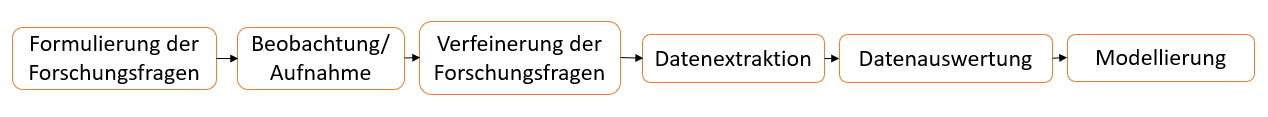
\includegraphics[width=1.0\textwidth]{pictures/introduction/strukture/strukture_work.png}
	\caption{Struktur des Vorgehens in bei der Modellfindung für diese Bachelorarbeit}
	\label{fig:Vorgehen}
\end{figure}
 
\section{Begriffe und Definitionen} \label{Begriffe und Definitionen}
Im Folgenden werden Begriffe definiert, die ich verwende, um den Fahrgastwechsel zu beschreiben. 
\begin{longtable}{ l p {10 cm}}
			 \textbf{Aussteiger}	& Personen die vom Inneren des Zuges auf den Bahnsteig gelangen wollen.\\
			 	& \\
			 \textbf{Einsteiger}	& Personen die vom Bahnsteig in das Innere des Zuges gelangen wollen.\\
				& \\
			 \textbf{Platzmacher}	& Personen, die aus dem Zug aussteigen, um anderen Personen im Zug die Möglichkeit zu geben auszusteigen. Diese Personen wollen danach wieder in den Zug gelangen.\\
				& \\
			\textbf{Türbereich}	& Bereich zwischen den Türen des Zuges, der beim Ein- und Aussteigen betreten werden muss. Siehe \figurename \ref{fig:Doorarea}\\
				& \\
			\textbf{Fahrgastwechselzeit}	& Die Zeit, die es dauert, bis der Fahrgastwechsel beendet ist. Der Fahrgastwechsel beginnt, wenn der erste Aussteiger den ersten Fuß auf den Bahnsteig setzt. Ist kein Aussteiger vorhanden oder existiert eine Person die einsteigt, bevor der erste Aussteiger mit dem Aussteigen beginnt,  so beginnt der Fahrgastwechsel, wenn der erste Einsteiger einen Fuß in den Wagon setzt. Der Fahrgastwechsel ist beendet, wenn der letzte Einsteiger seinen zweiten Fuß in den Wagon setzt. Falls keine Einsteiger vorhanden ist, oder noch ein Aussteiger aus dem Zug tritt, wenn schon alle Einsteiger im Wagon sind, wird der Fahrgastwechsel beendet, wenn der letzte Aussteiger seinen zweiten Fuß auf den Bahnsteig setzt.\\
				& \\
			\textbf{Prozesstypen}	& Einsteiger, Aussteiger und Platzmacher bilden die verschieden Prozesstypen.\\
				& \\
			\textbf{Personen}	& Wird in dieser Bachelorarbeit in Bezug auf den Fahrgastwechsel das Wort "`Personen"' verwendet ist damit immer die Gesamtheit der Personen gemeint, die an dem Fahrgastwechsel beteiligt sind. Also die Summe aller Einsteiger, Aussteiger und Platzmacher dieses Wechsels.
\end{longtable}

 \begin{figure}[H]
	\centering
		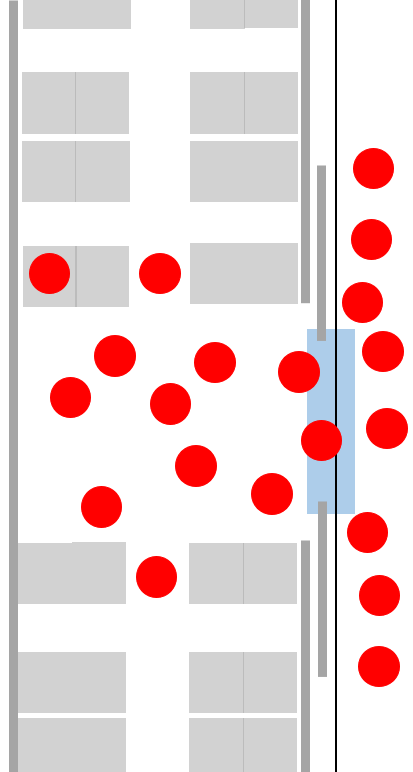
\includegraphics[angle=270, width=0.5\textwidth]{pictures/introduction/defenitions/example_doorarea.png}
	\caption{Skizze zur Erklärung des Begriffes "`Türbereichs"' aus der Vogelperspektive: U-Bahn "`Wände"' dargestellt durch graue Linien, Sitzplätze der U-Bahn durch graue Vierecke, Bahnsteigkante durch schwarze Linie, Fahrgäste durch rote Kreise. Der Türbereich ist durch ein blaues Rechteck gekennzeichnet.}
	\label{fig:Doorarea}
\end{figure} 
\todo{Überprüfen alle Begriffe definiert}
\section{Formatierung}
\begin{table}[H]
	\centering
		\begin{tabular}{ l p {12 cm}}
		\textsf{Sans Sherif}	& Schriftart wird verwendet, um Software zu beschreiben. Sie wird eingesetzt, wenn der Name einer Software verwendet wird.\\
		\texttt{Typ<ewriter}	& wird für Namen bei der Auswertung verwendeter Python Bibliotheken und Funktionen benutzt. \\
		\textsl{Slanted}	& wird bei Verweisen auf Zusatzmaterial verwendet, Dateiname wird dabei mit dieser Schriftart geschrieben.
		\end{tabular}
\end{table}